\documentclass[11pt]{sdm}
\usepackage{graphicx}
\usepackage{hyperref}

%numeroter les pages
\pagestyle{plain}

\title{Segmentation and recognition of symbols for printed and handwritten music scores}
\author{Kwon-Young \textsc{Choi}}
\usepackage[T1]{fontenc}
\usepackage[utf8]{inputenc}
\supervisorOne{Bertrand \textsc{Coüasnon}}
\supervisorTwo{Yann \textsc{Ricquebourg}}
\teamOne{Intuidoc Irisa France}
\supervisorThree{Richard \textsc{Zanibbi}} % ne fait pas partie de irisa, mettre RIT USA
\teamTwo{RIT USA}
%One of:
% ens-Rennes  esir    insa-rennes logoENIB  rennes1  UBO
% enssat header logo_ENIB   logoUbs   tel-br supelec

\school{logo_ENIB}


% the domain should be one or two of:
% Technology for Human Learning
% Artificial Intelligence
% Computer Arithmetic
% Hardware Architecture
% Automatic Control Engineering
% Bioinformatics
% Biotechnology
% Computational Complexity
% Computational Engineering, Finance, and Science
% Computational Geometry
% Computation and Language
% Cryptography and Security
% Computer Vision and Pattern Recognition
% Computers and Society
% Databases
% Distributed, Parallel, and Cluster Computing
% Digital Libraries
% Discrete Mathematics
% Data Structures and Algorithms
% Embedded Systems
% Emerging Technologies
% Formal Languages and Automata Theory
% General Literature
% Graphics
% Computer Science and Game Theory
% Human-Computer Interaction
% Computer Aided Engineering
% Medical Imaging
% Information Retrieval
% Information Theory
% Ubiquitous Computing
% Machine Learning
% Logic in Computer Science
% Multiagent Systems
% Mobile Computing
% Multimedia
% Modeling and Simulation
% Mathematical Software
% Numerical Analysis
% Neural and Evolutionary Computing
% Networking and Internet Architecture
% Operating Systems
% Performance
% Programming Languages
% Robotics
% Operations Research
% Symbolic Computation
% Sound
% Software Engineering
% Social and Information Networks
% Systems and Control
% Image Processing
% Signal and Image Processing
% Document and Text Processing
% Web
\domain{Domain:  Document and Text Processing, Computer Vision and Pattern Recognition}

%write your abstract here
\abstract{write your abstract here}



\begin{document}
\maketitle

%*****************************************************************%

\section{Introduction}

The research team Intuidoc from the Irisa laboratory has developed a generic way of recognizing structured documents by using the DMOS system.
The goal of this internship is to improve this generic document recognition method on the specific use of Optical Music Recognition (OMR).
The team has already formalized music notation grammar into rules understandable by the DMOS system.
But there are still problems during the low-level image recognition task.
Indeed, because of the density of information in a musical score and because of all pre-processing phases applied to the image, there are often cases of broken and overlapping musical symbols.
Currently, the recognition system used in DMOS is having difficulties in recognizing such symbols.
Therefore, the specific purpose of this internship is to improve the recognition of broken and overlapping symbols.

The hypothesis that will guide this bibliography is that by avoiding explicit segmentation during the recognition phase, we will be able to improve the recognition task.
In a way, we are following the history of Optical Character Recognition (OCR) and Speech Recognition where we have first used techniques with explicit segmentation, but now we have developed techniques that integrate segmentation in the recognition task.
Following state of the art techniques in OCR, Speech Recognition and Object Recognition, Neural Network provide powerful architectures that integrate implicit segmentation naturally.
Making generic methods are an important characteristic of the DMOS philosophy, so although we are working on music score, the improvement proposed should work for other structured documents.

We will first review the state of the art of OMR in section \ref{sec:soa_OMR} by first introducing how a music score is structured, then we will review the state of the art of OMR by presenting all steps classically used in OMR at section \ref{ssec:omr_steps}: pre-processing, staff removal, segmentation and recognition of music symbols, music notation reconstruction.
In a second section \ref{sec:merge}, we will review different techniques that may improve the segmentation and recognition of music symbols.
We will start with techniques that merge the segmentation and recognition task: Hidden Markov Model, Multi-Dimensional Long Short-Term Memory Recurrent Neural Network.
It is also interesting to study how the data is prepared for training and using the network.
Consequently, we will review how the A2IA team implemented a full document recognition chain in \ref{ssec:maurdor}.
Finally in section \ref{sec:object}, we will present other techniques used in Object Recognition like Deep Neural Network and a model of Visual Attention.

\section{State of the art of Optical Music Recognition} \label{sec:soa_OMR}

In this section we will first define what is Optical Music Recognition and its main issues.
Then we will describe all the steps commonly used for implementing an OMR system.
Finally, we will also briefly introduce the DMOS system developed by the Intuidoc team in the context of OMR.

\subsection{Definition}

Nowadays, digitalizing scores is a common practice to save and share music.
But the format of these documents cannot be directly interpreted by a computer.
That is why we have developed Optical Music Recognition systems for converting an image of a score to a format that is understandable by a computer.
This computer vision task could be therefore classified as a hybrid domain between Optical Character Recognition and image recognition.
OMR is principally used to save time because manually transcribing a score in machine readable format is very time consuming.
Many music composers still find awkward to directly write music with a music composer software and prefer to write their music on paper.
The use of OMR in these situations could integrate into the working flow of music composer their habit to write music on paper and automatically transcribe them in a computer readable format.

A score is a structured document used to formalize music.
Its organization is hierarchical, for example:
\begin{itemize}
  \item Different staves are used for different instruments or voices;
  \item Each staff contain five lines;
  \item A staff contains music symbols;
  \item A music symbol like a note is constructed by the association of graphical primitives like a dot, stem and flags \ldots
\end{itemize}
There are multiple symbols in musical notation resumed in figure \ref{list_symbols}: clefs, notes and rests, breaks, accidentals and key signatures, time signatures, dynamics \ldots 
\begin{figure}[btp]
  \centering
  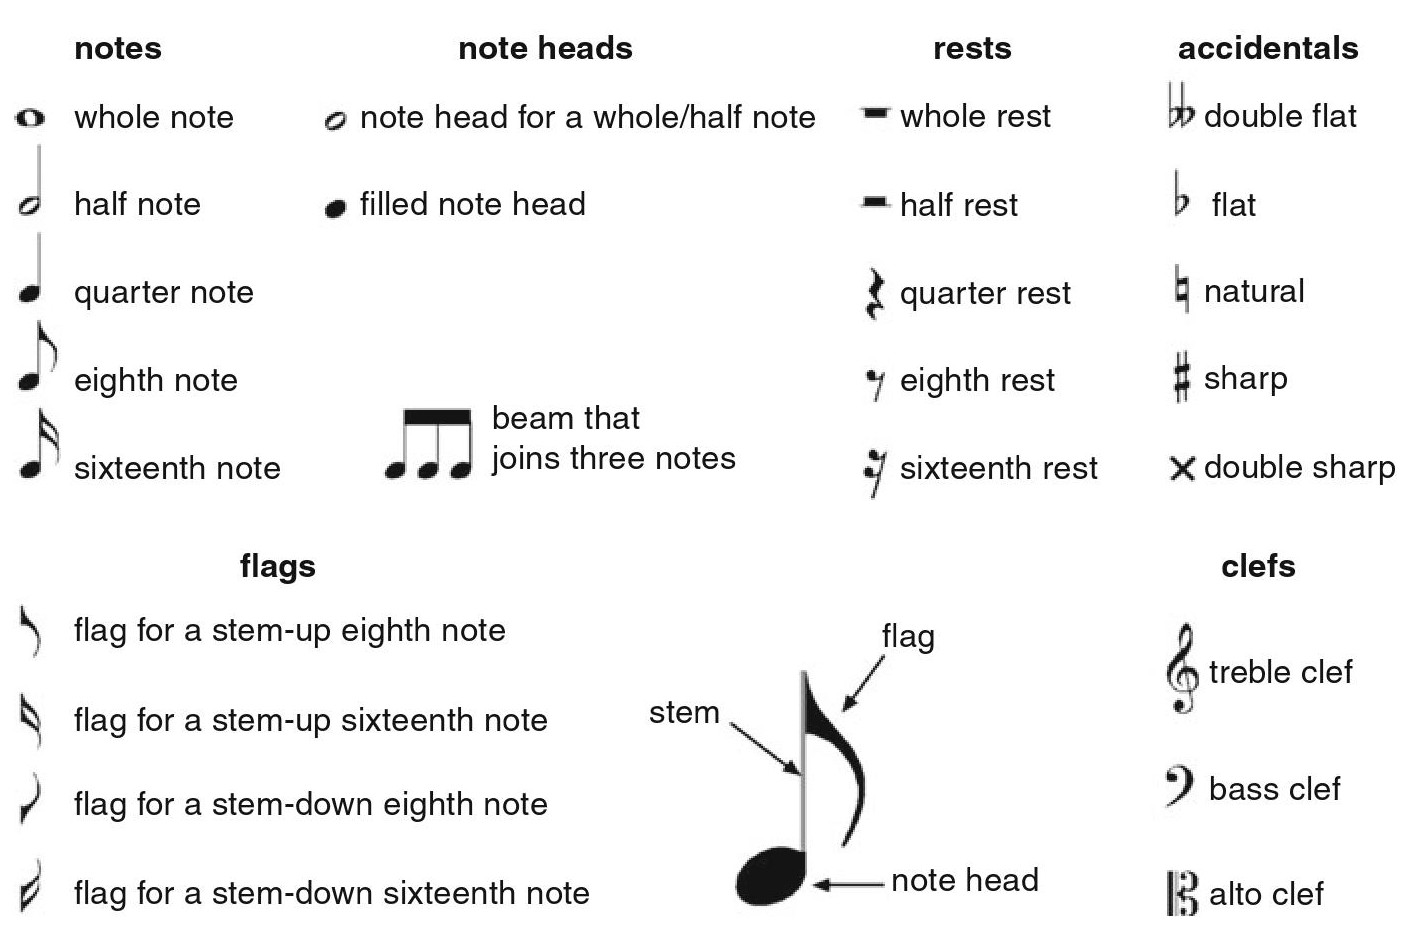
\includegraphics[scale=1]{img/list_symbols}
  \caption{\label{list_symbols} Non-exhaustive list of musical symbols \cite{fornes_analysis_2014}. }
\end{figure}

OMR systems are faced with multiple problems such as:
\begin{itemize}
  \item The high density of symbols;
  \item High connectivity between symbols;
  \item High variation of symbols;
  \item Overlapping and broken symbols like in figure \ref{connected_symbol}.
\end{itemize}
\begin{figure}[btp]
  \centering
  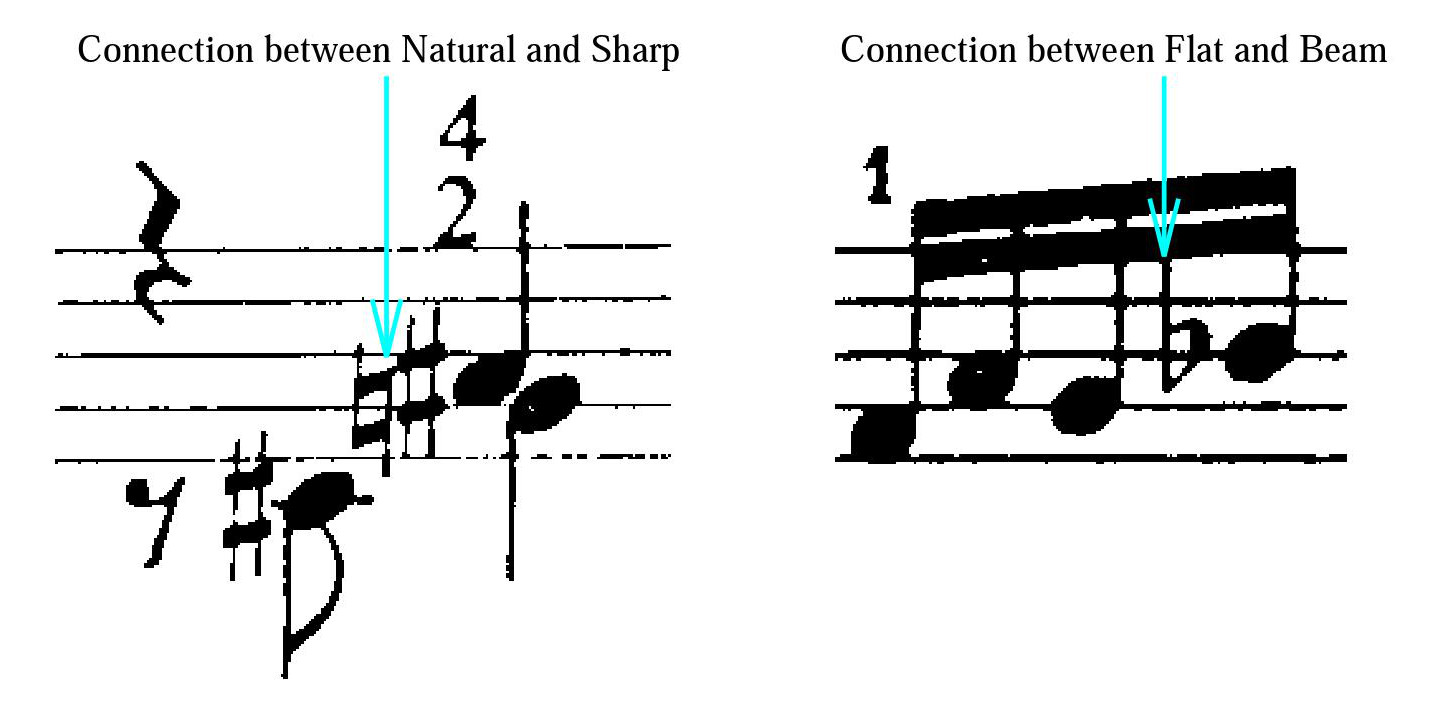
\includegraphics[scale=1]{img/connected_symbol}
  \caption{\label{connected_symbol} Examples of symbols that should not touch \cite{couasnon_using_1995}. }
\end{figure}
A score has a unidirectional direction of reading that corresponds to the time flow, but multiple things can happen simultaneously.
For example, when there is multiple instruments in the same score, all music symbols are vertically synchronized across staves.% as illustrated in figure \ref{vertical_synchro}.
%\begin{figure}[btp]
  %\centering
  %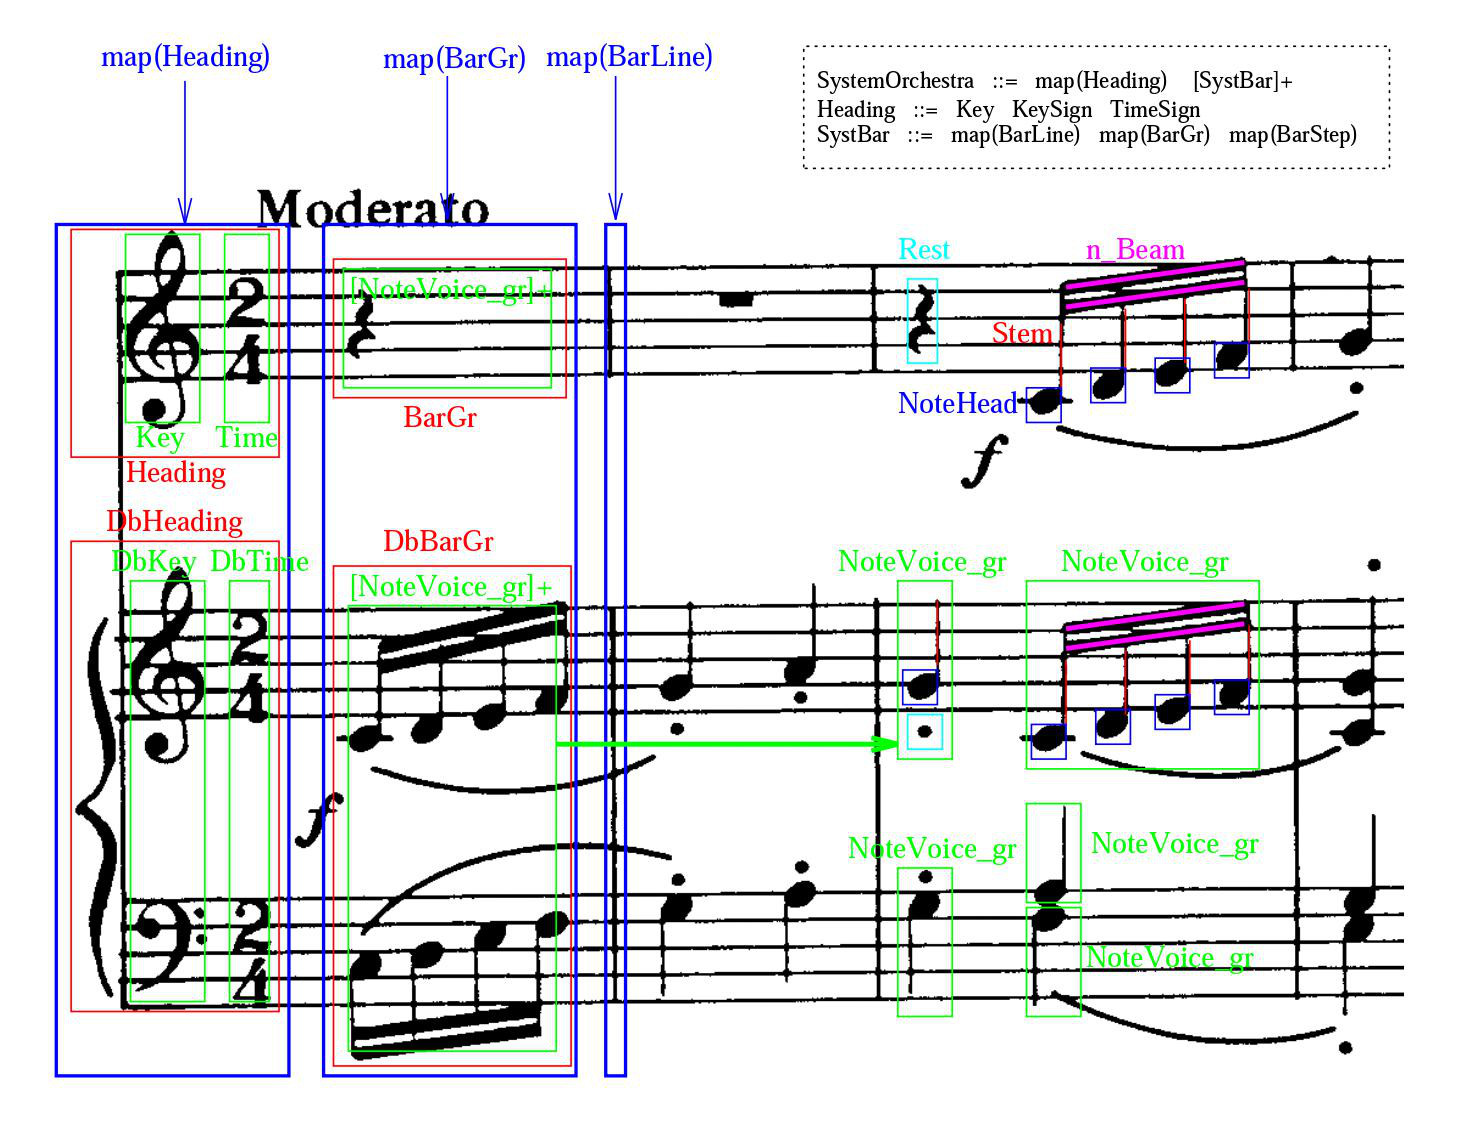
\includegraphics[scale=1]{img/vertical_synchro}
  %\caption{\label{vertical_synchro} Vertical synchronization of a score \cite{couasnon_using_1995}. }
%\end{figure}
As a consequence, the output of an OMR system is not just a one dimensional sequence of symbols.
All graphical symbols must be localized horizontally and vertically in order to deduce their relations between each other.

Authors like in \cite{rebelo_optical_2012} or \cite{fornes_analysis_2014} generally describe an OMR system by identifying multiple steps: pre-processing, staff removal, symbol segmentation, symbol recognition, music notation reconstruction.
A typical architecture of an OMR system is resumed in figure \ref{typical_omr} at page \pageref{typical_omr}.
We will first review all these different steps, however we can already point out that an OMR system constituted of these sequential steps is very limited because the segmentation and recognition is done without using the context.
That's why we will also present more in details the DMOS system at the end of this part because of its special architecture that can use the context for segmenting and recognizing music symbols.
Also, we will particularly focus our attention on symbol segmentation and recognition because it is the central theme of this internship.
\begin{figure}[btp]
  \centering
  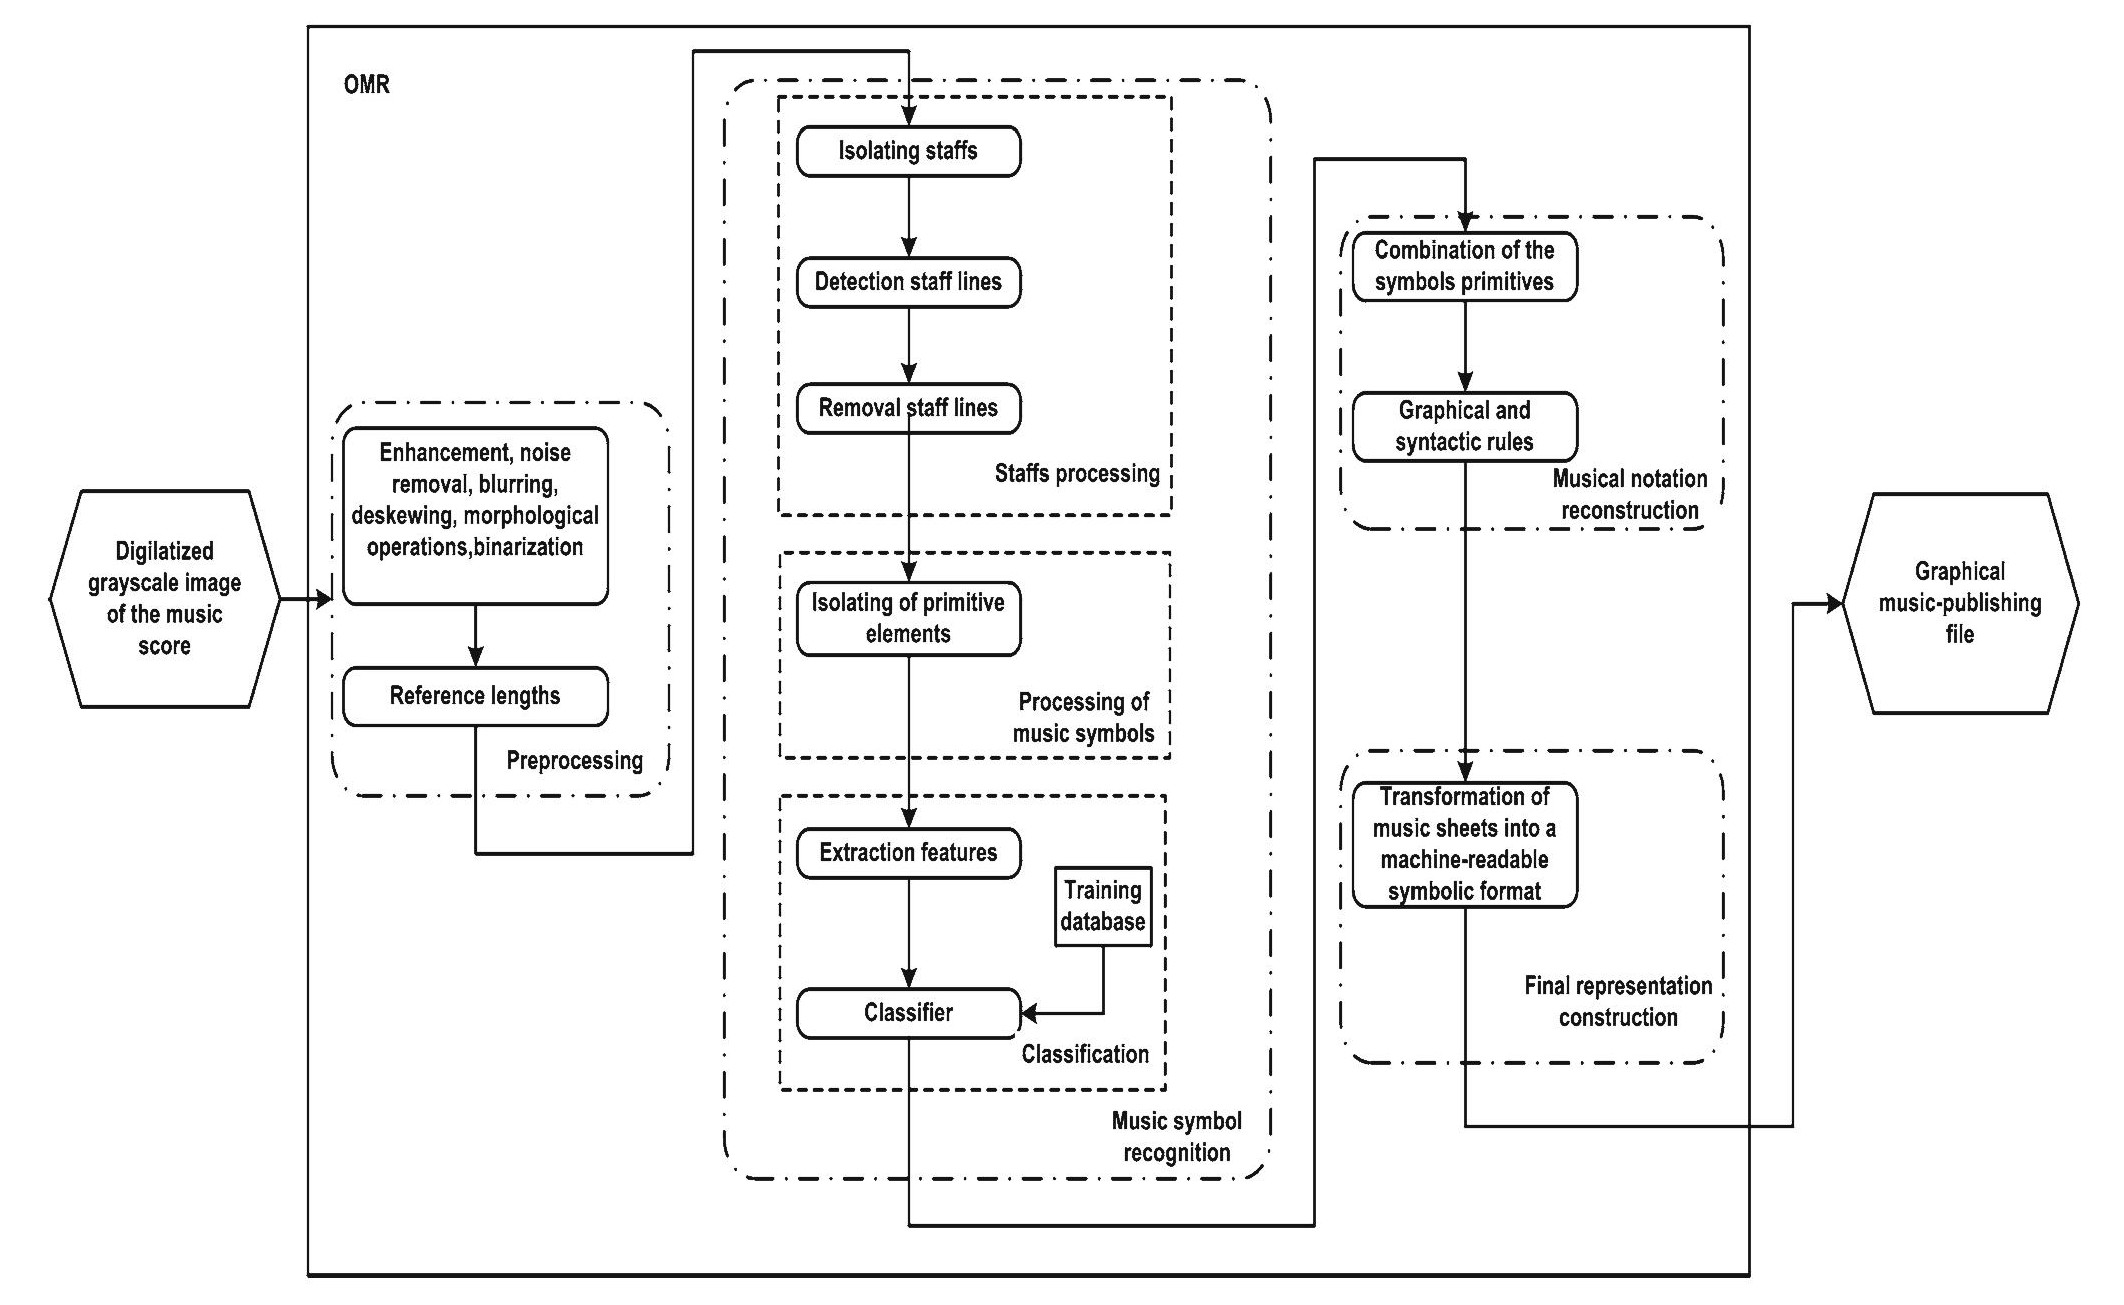
\includegraphics[scale=0.8]{img/typical_omr}
  \caption{\label{typical_omr} Typical architecture of an OMR system \cite{rebelo_optical_2012}. }
\end{figure}

\subsection{Different step of OMR} \label{ssec:omr_steps}

\subsubsection{Pre-processing}

The pre-processing phase of OMR consists of making some operations on the raw image to ease the latter steps of OMR.
Before anything, the image has to be converted into a binary image.
This operation is a classical step of computer vision tasks.
Then, optional operation can be applied to enhance the quality of the score.
\begin{itemize}
  \item Skew correction for staff line: used for simplifying the staff removal step;
  \item Noise removal for bad scanning and digitization, for example see the figure \ref{old_score} on page \pageref{old_score};
  \item Some other morphological operations \ldots
\end{itemize}

\subsubsection{Staff removal}

One characteristic of a music score is that most of the symbols are connected by the five lines that constitute a staff.
These lines are an obstacle for almost every classical technique of segmentation and recognition used in computer vision.
This is why, most OMR systems first remove these lines.

A fast way to do this is to do a horizontal projection of a music staff.
The resulting vertical position of an intensity peak is an indicator of the position of a line.
It is worth noting that these kind of projection or run length techniques do not deal well with overlapping symbols, and often result in breaking symbols.
Candidate assemblage and contour tracking are another way to remove a staff that are relatively fast to compute and can sometimes deal with overlapping symbols.
Graph path search techniques can produce really good results, but are slow to compute.
Finally, detection of lines in an image can be done by using complex filters like a Hough transform or a Kalman filter like the one used in the DMOS system \cite{couasnon_dmos_2001}.
The Kalman filter used in DMOS has the capability to recognize curved line, useful to detect hand written line.

\subsubsection{Music symbol segmentation and recognition}

\begin{figure}[btp]
  \centering
  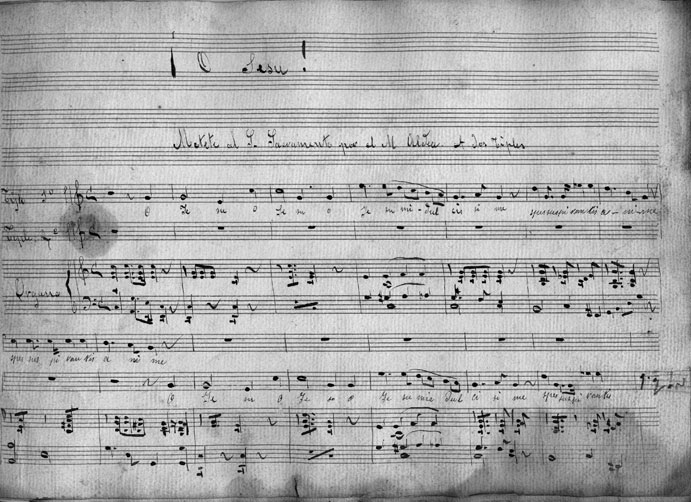
\includegraphics[scale=0.5]{img/old_score}
  \caption{\label{old_score} Old and damaged handwritten score \cite{fornes_analysis_2014}. }
\end{figure}
Music symbol segmentation and recognition are the core part of an OMR system.
It is also the more challenging part because of the high number and high variability of music symbols and its complex bi-dimensional structure.
This complexity is often aggravated because of bad digitalization and paper degradation for ancient scores like the figure \ref{old_score}.
Furthermore, symbols are often deteriorated because most of OMR systems do the staff removal step that often leads on breaking symbols.
Broken symbols then make the segmentation steps more challenging, even more if the context information is not taken into account.

Techniques used by OMR systems during this step are very diverse and many solutions have been proposed.
However, most of OMR systems first does a segmentation step and then apply recognition techniques to extract the correct symbol.
A simple way of segmenting a score is by first extracting graphical primitives like lines, blobs, circles \ldots and then joins these graphical primitives for the recognition stages.
Symbols can be extracted and recognizeed by using template matching techniques.
But these kind of techniques have many drawbacks as they are slow to compute and have a really low robustness when recognizing a symbol.
One way to recognize a symbol from a bounding box candidate is by computing simple operation that will result in simple features of the region of interest and then compare these features with those same features computed from symbols models.
This same philosophy can be used with different techniques by using symbol descriptors like centroids, Zernike moments, and decision trees.

The use of classifiers is yet another method to recognize a music symbol and four of them are compared in \cite{rebelo_optical_2009}.
Hidden Markov models have been extensively used for optical character recognition and speech recognition.
In \cite{pugin_optical_2006}, they have attempted to apply a hidden Markov model for recognizing very simple and old scores.
Their proposition has the interesting property to merge the segmentation task and the recognition task.

In the contrary, a prior segmentation is needed before the recognition can take place in the following classifiers.
This constraint is very limiting because many errors can happen in the segmentation phase because of broken and overlapping symbols.
Indeed, the use of the context is essential in correctly segmenting a music symbols.
The use of simple neural networks like a multi-layered perceptron also have been reviewed for recognizing music symbols.
The classic backward-propagation algorithm has been used for the training algorithm.
The results were disappointing as they were outperformed by some simple classifiers as the k-NN classifiers.
Nowadays, new neural network architectures have been proposed in similar domain like OCR, Speech Recognition or Computer Vision, but to our knowledge, they have never been used in the field of OMR.
The k-nearest neighbor algorithm used in this context is the simplest classification algorithm used.
They implemented it using Euclidean distance and it gave the second best result after the Support Vector Machine (SVM) classifiers.
SVM used a radial basis function network and at the time of the study, it was the classifier that gave the best result.
For this internship, we are looking for new ways of recognizing broken and overlapping symbols and one of our hypothesis is that by merging the segmentation and recognition phase, we will improve the recognition rate.
That is why we will review more in detail the HMM proposition later in this work, see section \ref{ssec:HMM}.

\subsubsection{Music notation reconstruction}

The music notation reconstruction has the specific task to interpret the spatial relationship between different primitives or symbol recognized.
This kind of algorithm has to deal with the complex two dimensional structure of music notation.
As a consequence the positional information of a music symbol is very important as well as the context of the symbol.

OMR system has used fuzzy models or grammars to formalize musical notation.
We can differentiate two kinds of grammars.
Rule based grammar, or graph based grammar.
Most of the systems that use a grammar for formalizing the music grammar are only using an ascending recognition methods.
All steps of preprocessing, staff removal, symbol segmentation, symbol recognition and finally music notation reconstruction using a grammar take place sequentially and therefore limit the use of the context in the segmentation and recognition phase.
In this work, we will focus on rule based grammar by presenting the DMOS system \cite{couasnon_dmos_2001} as it is the system that will be used during this internship.

\subsection{DMOS: a generic document recognition method}

DMOS, "Description and MOdification of Segmentation", is a general method for the recognition of structured documents.
Its main purpose is to separate the semantic and graphic knowledge of the program that do the recognition task because of the well-known paradox in computer vision that there is a "discrepancy between the way knowledge describe an object and the way objects have to be recognized" \cite{couasnon_dmos_2001}.

The system implemented in \cite{couasnon_dmos_2001} is mainly separated in two parts.
First, the system uses a grammar for formalizing the semantic and graphical organization of the documents.
This grammar is derived from the EPF grammar (Enhanced Position Formalism) and is expressed in a Prolog dialect called $\lambda Prolog$.
There are two levels of grammar:
\begin{itemize}
  \item A physical level: formalization of the graphical organization of the documents;
  \item A logical level: work on the semantic level of the document.
\end{itemize}
The grammar manipulates \textit{terminals} that are simple graphical units like a line or a little connected component.
It’s by agglomerating these terminals that the grammar construct complex structures that will describe the graphical and the semantical organization of the document.

The second part is where the originality of the approach is found.
A classical computer vision system that uses a grammar only uses it at the end of the recognition chain.
First, some tools for segmenting and recognizing a symbol is used.
Then, labels recognized are fed into the grammar for detecting possible recognition errors and performing the reconstruction of the semantic notation of the document.
In the DMOS system presented by \cite{couasnon_dmos_2001}, the grammar totally guide the segmentation and recognition of the document.
This grammar decides on how to segment the document, then feed the candidates into classifiers that will confirm the label of the candidate.
The grammar can then check if the recognition is consistent, and if it is not, it can redo the segmentation step for finding a better solution.
The grammar can therefore use the context for segmentation \textit{and} recognition tasks.

This system has been initially implemented for recognizing orchestral scores and has been validated on the task of recognizing around 5000 old military forms.
For validating the modelling capacity of DMOS and its advantageous use of the context, this method has been initially implemented for recognizing orchestral scores.
Furthermore, this system has been applied and validated on more than 700 000 heterogeneous and complex documents of numerous different types: archive documents, handwritten letters, forms, papers, tables, mathematical formulae \ldots
However, this system is still having difficulties in recognizing broken and overlapping symbols in scores.
Since the proposition of the orchestral scores recognition using DMOS, many new techniques in computer vision for the segmentation and recognition task have been found.
We will now review some of those techniques.

\section{Merging recognition and segmentation phase for symbol classification} \label{sec:merge}

Our hypothesis is that by merging the segmentation task at the symbol level, we will improve the recognition rate of our system.
An attempt has been made in this direction by using a Hidden Markov Model for recognizing old and very simple scores.

\subsection{Hidden Markov Model applied to OMR} \label{ssec:HMM}

Authors in \cite{pugin_optical_2006} present a Hidden Markov Model for recognizing old and very simple scores as show in figure \ref{old_score_HMM}.
They decided to avoid the staff removal step and the segmentation step because they considered that these steps are important sources of errors.
They trained their model with a dataset of 240 pages of music scores containing 175 symbols.
The partitions were manually annotated with graphical information.
The recognition process used imitates speech recognition as they used a sliding window for scanning the score.
They simplified the problem by only having a succession of notes from left to right.
As a consequence, their system couldn't handle chords because the model was sequential and unidirectional.
They computed 4 to 40 features from the raw score image and used the Baum-Welch algorithm for training the HMM.
The recognition rate obtained was around 96\% but this rate is highly dependent on the feature chosen, the sliding window width, \ldots

This method has the advantage to avoid explicit segmentation by using a Hidden Markov Model.
But this model will be hard to be applied to more complex scores as they have simplified the problem by using only unidimensional scores.
Indeed the objective of this internship is to work on bigger and complex orchestral scores.
The HMM is also known for having difficulties to use context information because of their architecture principle.
This is why, we will introduce next another architecture used on Optical Character Recognition and Speech Recognition that avoid totally the segmentation during the training phase and have no problem with using long-term dependency information.
\begin{figure}[btp]
  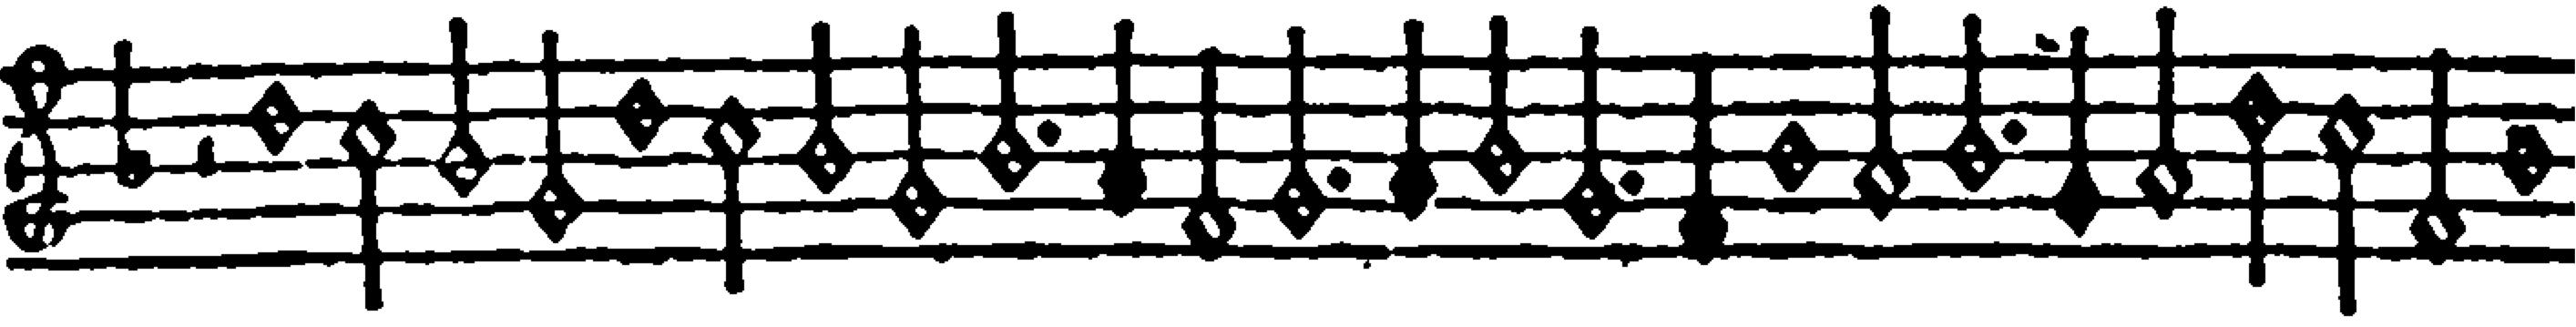
\includegraphics[scale=0.16]{img/old_score_HMM}
  \caption{\label{old_score_HMM} Example of old score recognized in \cite{pugin_optical_2006}. }
\end{figure}

\subsection{Recurrent Neural Network applied on OCR and Speech Recognition}

In the Optical Character Recognition field, a new kind of architecture has been presented by Graves and Schmidhuber \cite{graves_offline_2009}.
They used Long Short-Term Memory Recurrent Neural Network (LSTM RNN) \cite{hochreiter_long_1997} for dealing with long term dependency.
The contextual information has been handled by a Multi-Dimensional Recurrent Neural Network (MD RNN) and they avoided explicit segmentation by using a Connectionist Temporal Classification (CTC) output layer \cite{graves_connectionist_2006}.
An image is not just a one dimensional sequence of data needed for the input of the CTC, so they used a specific type of architecture for reducing a two dimensional image to a one dimensional sequence.

\subsubsection{Long Short-Term Memory Recurrent Neural Network (LSTM RNN)}

RNN is a type of neural network that are designed to recognize sequences of data.
However, simple RNN are known for having the vanishing and exploding gradient problem.
Indeed, when training a RNN with the classical gradient descent algorithm, each time-step is like a new layer of the network, making it a very deep network.
Long Short-Term Memory Recurrent Neural Network presented in \cite{hochreiter_long_1997} is designed to resolve this problem.

To control the variation of the gradient, they truncate the gradient during the training phase.
They used a "constant error carrousels" to ensure constant error flow through the network.
The base unit of the network is not anymore a neuron, but a memory cell constituted of two gates, see figure \ref{lstm_unit}.
First, a multiplicative input gate unit to protect the memory stored in the unit from irrelevant input.
Second, a multiplicative output gate used to protect other units from the irrelevant memory of the unit.
Later papers have proposed variation of this architecture by adding gates like a forget gates to erase the memory of the unit.
Each of these units has to be properly trained to respectively learn which error to release or to keep.

In \cite{hochreiter_long_1997}, they presented this kind of RNN using three fully connected layers: one input layer, one hidden layer, one output layer.
They applied it in multiple experiment like learning the "embedded Reber grammar" or other sequence.
They showed that LSTM can handle very long time lag, is very robust to noise and can generalize well.
The main advantage of the LSTM RNN is to be able to deal naturally with long-term dependency in the data sequence.
Next we will see how to use the context when working with two dimensional data like an image.
\begin{figure}[btp]
  \centering
  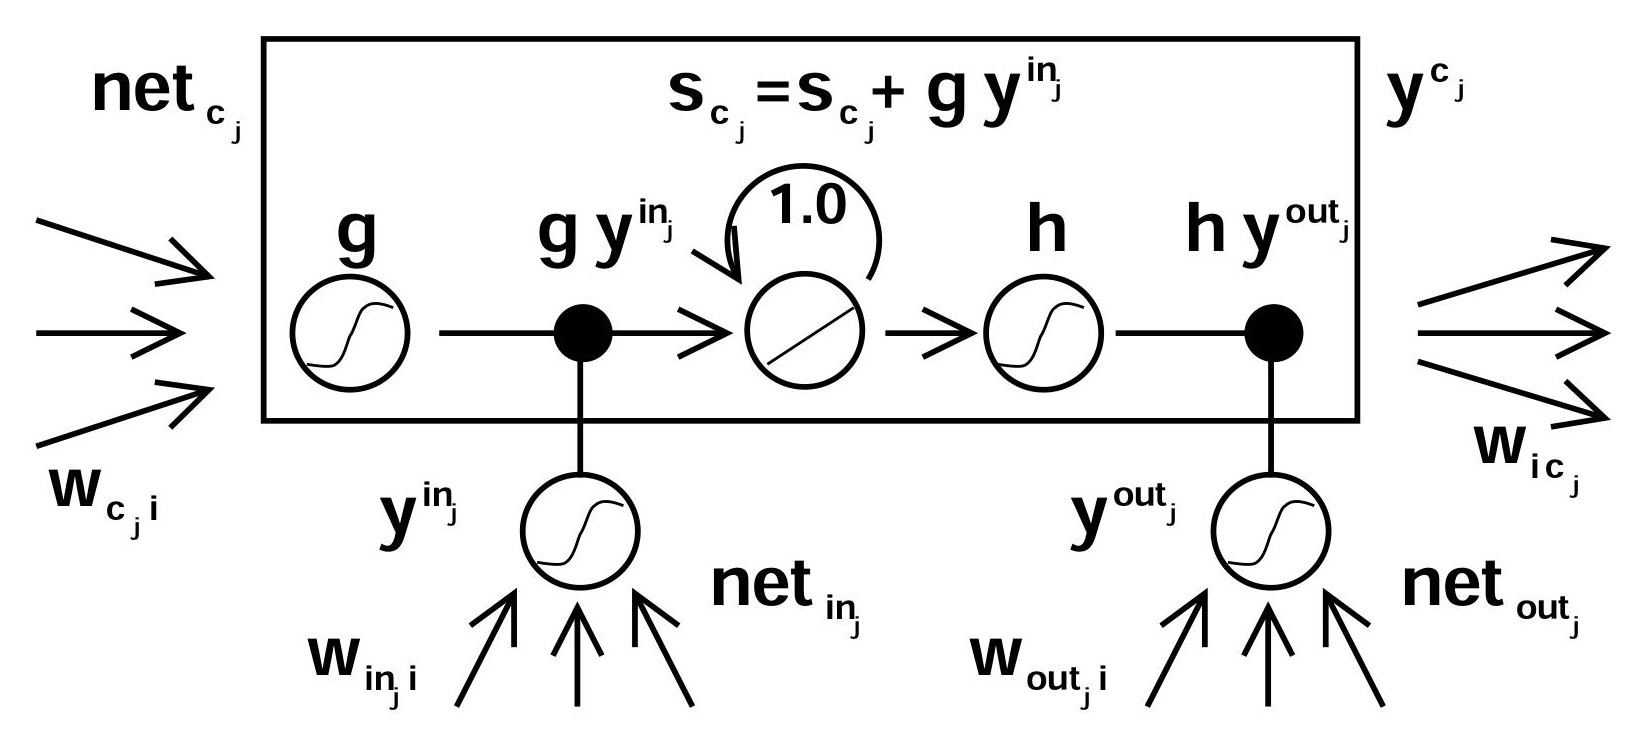
\includegraphics[scale=1]{img/lstm_unit}
  \caption{\label{lstm_unit} Architecture of a memory cell \cite{hochreiter_long_1997}. }
\end{figure}

\subsubsection{Multi-Dimensional Recurrent Neural Network (MD RNN)}

The novelty presented in \cite{graves_offline_2009} is the use of Multi-Dimensional RNN.
This network is a generalization of the Bi-Directional Neural Network presented in \cite{schuster_bidirectional_1997}.
Bi-directional Neural Network is used for handling past and future context for 1 dimensional data by adding recurrent connections to the previous sample and the future sample.
Similarly, MD RNN generalize this principle for N dimensions.
For example, an image is a two dimensional data, so a MD RNN used on an image adds 4 recurrent connections in all spatial directions.
To do this, \cite{graves_offline_2009} describe a four layer network where each layer scans from each corner of the image.
This way, it allows the network to create a flexible internal representation of the surrounding context.
Furthermore, this kind of networks are very robust to local distortion, making it an ideal system for recognizing handwritten data.
The MD RNN is trained with the backpropagation algorithm generalized to N dimensions.

This kind of network could be very interesting for recognizing musical symbols, especially handwritten symbols because of their robustness to distortion.
Furthermore, the context is extremely important for recognizing a symbol in a score.
However, it is still too early to say if this kind of network could learn the complex structure of a score.

\subsubsection{Labelling unsegmented sequence of data}

The work of \cite{graves_connectionist_2006} introduced the Connectionist Temporal Classification layer that allows a new way of training RNN for labelling unsegmented sequence of data directly.
The CTC layer is an output layer designed for one dimensional sequence labelling.
The principle is to train the network to estimate the conditional probabilities of all the possible labelling.
If the alphabet used during a recognition contains N symbols, the CTC layer will contain N+1 symbols because it adds the blank output.
The output of a CTC layer is normalized using a softmax function.
Then, all repetitions and blanks are removed to form blocks of symbols.
Training is done with the back propagation in time algorithm with the negative log probability function as the objective function.

The main advantage of this proposition is the fact that the whole network can be trained without pre segmenting the ground truth data, or post processing the output of the network.
However, in the context of OMR, the major problem is that the CTC layer is designed to label one dimensional sequence data, and we have already pointed out that a score is a complex two dimensional structure.
What we need from the output of an OMR system is the label of the symbol, but also his exact coordinates in the image.
This problem is further developed in the next section where the authors of \cite{graves_offline_2009} show how they transform an image into a one dimensional sequence of data.

\subsubsection{Network Hierarchy}

We will now present the overall hierarchy used in \cite{graves_offline_2009} for their OCR system.
The most common way for doing image recognition is not to directly work on the pixel level of the image, but to first extract \textit{features} of the image and then do the recognition phase.
A feature can be described as a small piece of information extracted from the image.
The authors use this same principle, however, they have a hierarchical approach for feature extraction.
This allows them to build complex visual properties of the raw image.
In computer vision, this kind of structure is called an \textit{inverted pyramid structure}: small layers at the bottom of the hierarchy and large layer at the top of the hierarchy for creating an efficient network.

The hierarchical structure is composed by interleaving MDLSTM layers with feedforward network.
Activations of MDLSTM layers are gathered into blocks.
The purpose of these blocks is mainly to provide a local contextual information and also to reduce the area of the activation arrays: at each level of the network, the vertical axis of the data is reduced to finally form a one dimensional sequence from a two dimensional block of data.
This is called \textit{subsampling}.
For the specific application of OCR, authors have found that three layers of MDLSTM/Feedforward give the best results.

This architecture has a dual property of reducing a two dimensional image into a one dimensional sequence and to be able to train and use the entire system without segmenting the data.
The first characteristic is not interesting in the context of OMR because we already said that a score is not a one dimensional sequence of data.
However, the second characteristic is very likely to improve the recognition of broken and overlapping symbols.
We will now see how this architecture can be used for complex recognition process as the Maurdor challenge, see the section \ref{ssec:maurdor}.

\subsection{Multi-lingual printed and hand-written text recognition system at the Maurdor evaluation} \label{ssec:maurdor}

We already highlighted the fact that OCR is a source of inspiration for OMR, but the main difference is that the structure to recognize is much simpler in OCR.
A score is a bi-dimensional structure with a notion of vertical synchronization and this notion is especially important for orchestral scores where there are many parallel staves for each instruments.
However, this is only true at the symbol level.
In fact, if we zoom out and consider an entire document, the recognition process can be much more complex.
For example, the Maurdor evaluation \cite{_maurdor_2016} is a computer vision and document recognition contest with some very hard data to recognize like the figure \ref{maurdor}.
The A2IA team has submitted an entire document processing chain and ranked first at the second Maurdor evaluation for both printed and handwritten text recognition for French, English and Arabic \cite{moysset_a2ia_2014}.
The document processing chain is composed of:
\begin{itemize}
  \item Document layout analysis;
  \item Write type identification;
  \item Language identification;
  \item Text recognition;
  \item Logical organization extraction;
  \item Information extraction.
\end{itemize}
They used a MD LSTM Recurrent Neural Network previously explained in the text recognition part, with little changes:
\begin{itemize}
  \item Adapted the sub-sampling filter size to fit the image resolution;
  \item Tuned hidden layer sizes for the dataset.
\end{itemize}
One important improvement to the training phase was the use of a powerful regularization technique called dropout.

However, the interesting part here is their technique to automatically prepare the data for the training phase.
Indeed, instead of just recognizing lines of text, a paragraph of text was given to the input of the text recognition module.
That's why they used an automatic system for the alignment of annotations and images of lines of text.
They used a line detection algorithm to extract lines of text and they applied a constrained line recognition system to match the lines image to a part of the ground-truth text.
In the context of this internship, we could also use the powerful grammar present in the DMOS system to roughly segment a score and spot zones with broken and overlapping symbols.
Then, we could feed these zones to a recognition system like the one we saw previously.
\begin{figure}[btp]
  \centering
  \includegraphics[scale=0.5]{img/maurdor}
  \caption{\label{maurdor} Example of a document from the Maurdor Challenge \cite{moysset_a2ia_2014}. }
\end{figure}

\section{Joint object localization and recognition techniques} \label{sec:object}

After reviewing some techniques used in OCR and Speech Recognition, it could be interesting to see what kinds of recognition systems are used for object recognition in an image.
Nowadays, deep neural networks are widely used in object recognition and are known to be the state of the art in image recognition \cite{erhan_scalable_2014}.
We will also review another proposition \cite{ba_multiple_2014} that concentrate on modelling an effective visual attention model.

\subsection{Deep Neural Network}

In \cite{erhan_scalable_2014}, they used a Deep Neural Network for detecting and localizing multiple scalable object in an image.
A common way to localize different object in an image is to train one object detector by class to recognize.
As the number of classes grows, it becomes computationally difficult to scale up the system.
The originality of this works is to train one single Deep Neural Network that is \textit{class agnostic} and use it to localize any object of interest in an image.
This Deep Neural Network is structured with multiple Convolutional Neural Networks and multiple max-pooling layers.
The output is normalized with a soft-max layer.
The recognition system proposed has the capability to output a bounding box to localize objects and a confidence score about the label of all objects detected.
The strength of this proposition is its property to handle naturally multiple instance of an object in an image.

In the context of OMR, this kind of network could be interesting as it can localize precisely with a bounding box an object in an image.
The fact that the bounding box is scalable is also interesting because there are multiple musical symbols that can be used at different sizes.
However, the training phase is still a problem, because training data still have to be graphically annotated to point the ground-truth location of the object.
In OMR, such database doesn't exist.
In fact, OMR database are not well developed.
There are some music symbols databases used for training simple classifiers.
Databases of image of music scores exist with often the semantical transcription of the score using the MusicXML format or the Midi format, but the graphical annotation of each symbol is not existent.

To attempt to address this problem, we will now introduce another use of RNN applied for Object Recognition.

\subsection{Multiple Object Recognition with Visual Attention}

\begin{figure}[btp]
  \centering
  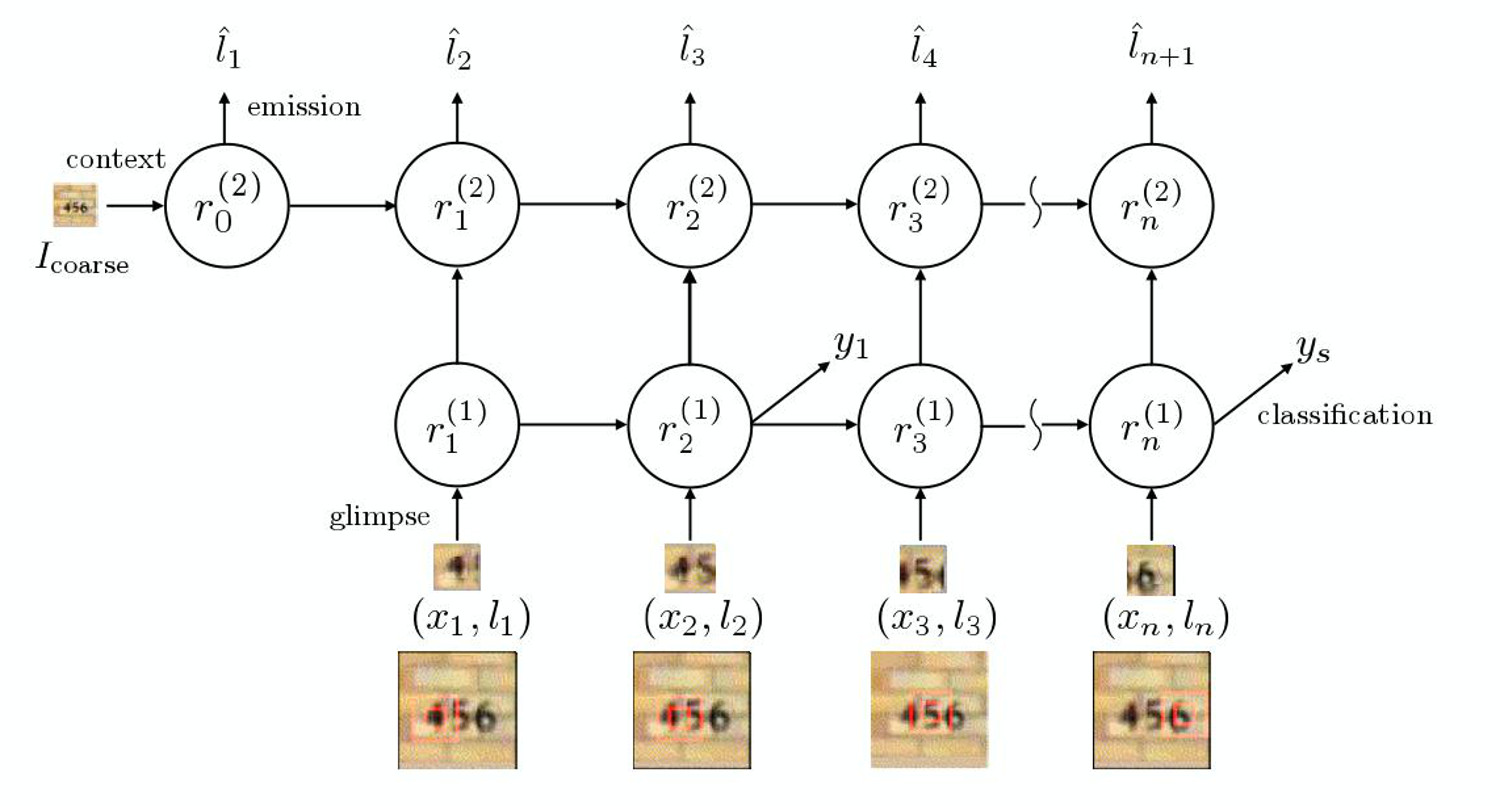
\includegraphics[scale=1]{img/attention_model}
  \caption{\label{attention_model} Deep recurrent attention model \cite{ba_multiple_2014}. }
\end{figure}

Authors of \cite{ba_multiple_2014} proposed an attention-based model inspired by the human vision with the purpose to recognize multiple objects in images.
Studies on human vision show that a human gradually construct its environment representation by focusing its attention on successive small parts of the image.
This principle is used here by using a Deep Recurrent Neural Network that processes an image by taking \textit{glimpse} at different resolutions.
A glimpse is a small part of the image centered on a special location.
Furthermore, they used reinforcement learning to train the network to learn about how to scan the image.
The model can learn to localize and recognize multiple objects, although it was only trained with class labels.
They evaluate the system by using this model to transcribe house numbers from Google Street View.
This model showed to be more accurate than state of the art convolutional networks, although the model is using fewer parameters and less computation.

The Visual Attention model process the image in N sequential steps.
For each step, the model scans a new location and extracts a glimpse at this location.
From this glimpse, the model updates its internal representation of the image.
The model uses a special classifier for recognizing objects.
Finally, the model output a new location to scan from.
The model is divided successively in sub-component and each of those components is a neural network.
The first network is the glimpse network used to extract features from the glimpse with two input layer: a convolutional layer that take a glimpse as an input and a fully connected layer that take the location of the glimpse as an input.
These two layers are then combined by multiplying the output of each layer.
The next network is a recurrent network composed of two recurrent layers composed themselves of LSTM units.
Its work is to aggregate information extracted from successive glimpses while preserving the spatial information.
Then a third network called the emission network is used to predict the location of the next glimpse.
A context network is used to compute an initial state of the system and provide the location of the first glimpse.
Finally a classification network is used to output a prediction from the RNN layer.
It is composed of a fully connected hidden layer and a softmax output layer.

This kind of model could be useful in our OMR system.
The fact that this model can locate and recognize symbol, although the network was only trained with class labels is interesting because in OMR, we only have databases containing class label symbols.
Furthermore, this system can locate an object in an image, making it ideal for an OMR system.
Without having this system to learn how to read a complex score, we could use the grammar to make a first rough segmentation and then use this recognition system for locating accidentals, key signatures, time signature, silences \ldots

\section{Conclusion}

A renewed interest is showing toward OMR in the computer vision and pattern recognition research field because it has still many challenges to overcome.
While OCR is now very advanced and has human like results, we still have many difficulties in recognizing music scores because of its complex structure and variety of symbols.
Many solutions have been proposed for every step of OMR: pre-processing, staff removal, music symbols segmentation and recognition, music notation reconstruction.
However, traditional OMR system that implement all these steps have an ascending architecture and imply many limitations.
First of all, the staff removal phase is often essential, but is very likely to damage symbols in the score.
Moreover, by applying all these steps sequentially, it is not possible to use the context during the segmentation and recognition phase.
The DMOS system is different because it is the grammar that guide the segmentation and recognition of the score.
As the system is constructing a representation of the score, it can reapply the segmentation and recognition phase to improve the overall recognition results.
The goal of this internship is to improve the segmentation and recognition phase of this DMOS system.

The main hypothesis of this study is that by avoiding explicit segmentation, we will be able to reach a better recognition rate.
An example of avoiding explicit segmentation has been done by using HMM on old and very simple scores.
But the history of OCR and speech recognition show us that after using HMM, state of the art systems use new found architectures of neural networks that have many interesting properties.
Especially Recurrent Neural Networks are providing a great way to avoid explicit segmentation by using a Connectionist Temporal Classification layer.
They also handle naturally long term dependency and therefore use the context to recognize symbols.
However, to the best of our knowledge, these networks have never been used in OMR, principally because of the fact that they are designed to recognize one dimensional sequence data.
During this internship, the major challenge will be to adapt this kind of architecture to recognize a music score.
We could imitate the A2IA team who first did a pre segmentation on a paragraph of text for extracting lines of text.
Similarly, this could be done by using the DMOS grammar to do a rough segmentation and therefore reduce a complex two dimensional structure into a simple one dimensional sequence of symbols.

Deep Neural Networks are also intensively used in object recognition and localization.
Their interesting property is that they naturally handle two dimensional information by providing bounding box to localize an object.
However, training data have to be graphically annotated and these kind of database is inexistent in OMR.
Finally, another approach using RNN is by using them with an attention-based model to guide the scanning process of the image, and therefore localize a symbol in a two dimensional space.
The use of complex neural network in OMR is very rare because authors prefer to rely on a bi-dimensional grammar to express the complexity of a music score.

In this internship, we will try to use both techniques by taking the best of both worlds.
Following the philosophy of DMOS, all the work that will be done in this internship should be applicable to any other structured documents.
This is why this internship is done in collaboration with Richard Zanibbi who also works on document and pattern recognition at the Rochester Institute of Technology.

%\section*{References}

\bibliographystyle{plain}
\bibliography{model}
\end{document}
%%% Local Variables:
%%% mode: latex
%%% TeX-master: t
%%% End:
